\documentclass[../Bachelorarbeit.tex]{subfiles}
\begin{document}
\chapter{Stand der Technik}
\label{chap:analyse}

Nachdem in Kapitel \ref{chap:einfuehrung} - \nameref{chap:einfuehrung} die ersten konkreten Überlegungen bis hin zu einem \nameref{sec:anwendungsszenario} aufgezeigt wurden um den Inhalt und die Funktionsweise des Prototypen zu umreißen, widmet sich dieses Kapitel der Domäne für die der Prototyp entwickelt wird.
Für diesen Zweck ist das Kapitel in zwei Abschnitte unterteilt. 
Im ersten Abschnitt (\nameref{chap:analyse:sec:sota}) wird ein Blick auf die Forschung und Fachliteratur geworfen, während sich der zweite Abschnitt (\nameref{chap:analyse:sec:analyBestehendeKonz}) mit echten Projekten beschäftigt, die eine Relevanz für den Prototypen darstellen.


\section{Literaturrecherche}
\label{chap:analyse:sec:sota}


\ideas{Einführung Themen aus der Entscheidungstheorie...Einzelne Punkte von Tufte, je nach Relevanz...Literaturrecherche ... sowie was aktueller Stand der Technik sowie Forschung.}



Daten OSM

\todoImprovement[]{weitere Analyse}
\todoInfo[]{Was ist gut, was ist schlecht?}

\section{Analyse von bestehenden Konzepten}
\label{chap:analyse:sec:analyBestehendeKonz}
\todoImprovement[]{Abschnittstitel konkretisieren}
\todoImprovement[]{Thema genauer ausarbeiten}


\subsection{Google Maps}
\label{chap:analyse:sec:sota:sec:google_maps}

\subsection{SmugMap}

\begin{figure}[t!]
\centering
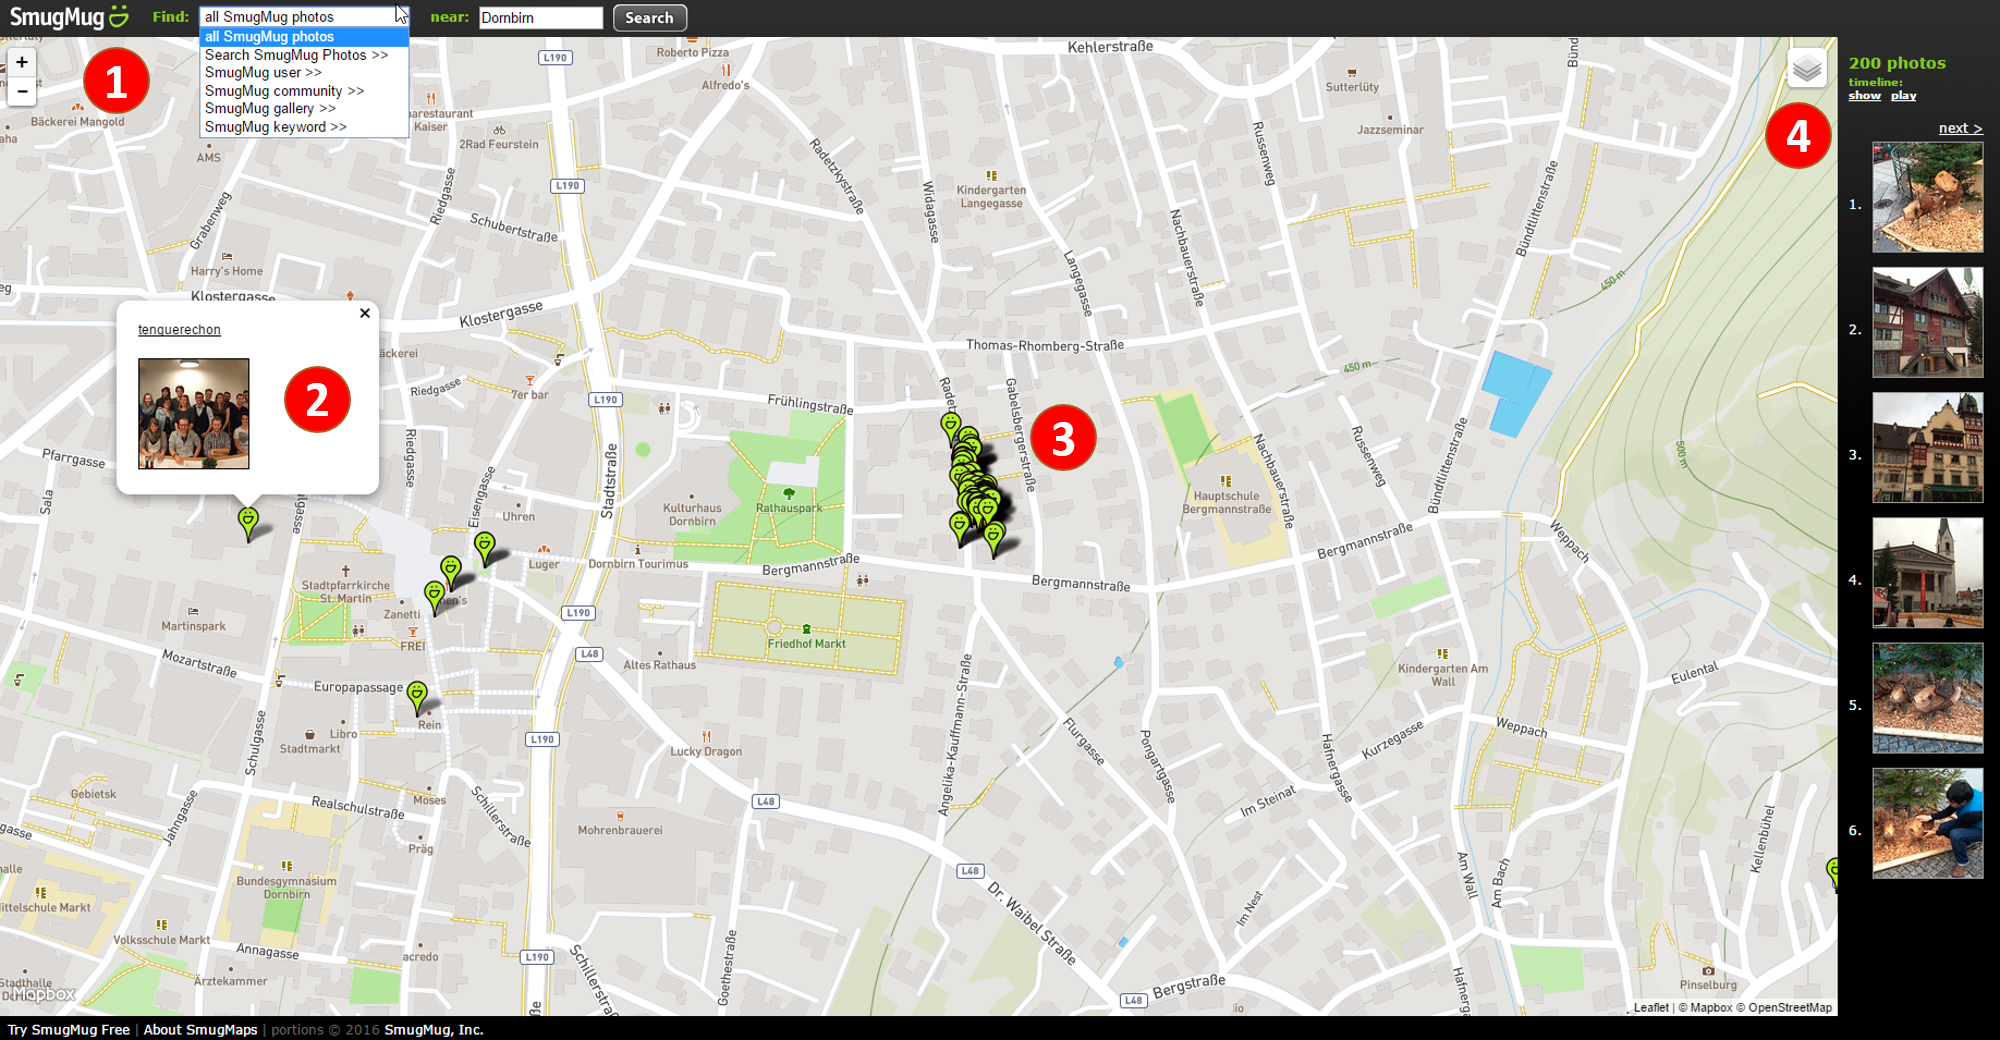
\includegraphics[width=1\linewidth]{img/StandDerTechnik/mapsSmugmugCom}
\caption[kurz]{Übersicht: Smugmug Map (Quelle: eigene Ausarbeitung | Daten und Kartenmaterial:http://maps.smugmug.com/)}
\label{fig:mapsSmugmugCom}
\end{figure}

\begin{figure}
\centering
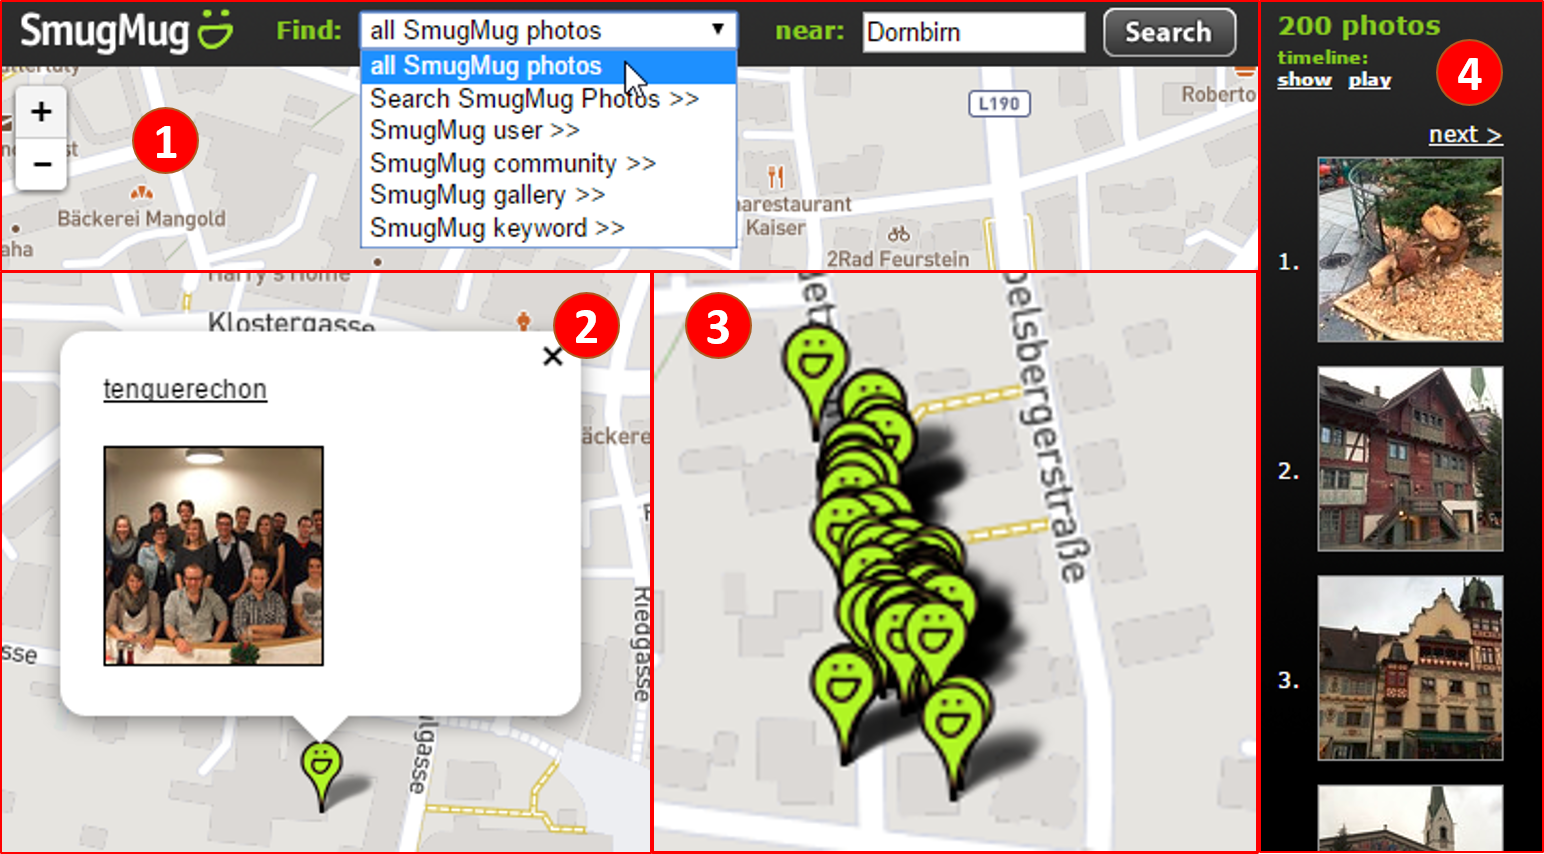
\includegraphics[width=1\linewidth]{img/StandDerTechnik/mapsSmugmugComDetail}
\caption[kurz]{lang Details der Smugmug Map (Quelle: eigene Ausarbeitung | Daten und Kartenmaterial:http://maps.smugmug.com/)/}
\label{fig:mapsSmugmugComDetail}
\end{figure}

\subsection{Airbnb}
Bei Airbnb handelt es sich um eine Webseite die sich auf die Vermittlung von Unterkünften spezialisiert hat\footnote{
	Airbnb ist unter der Addresse https://www.airbnb.at zu erreichen. Die getätigten Aussagen über die Webseite beziehen sich auf den Stand im Sommer 2016.
	}. 
Dabei können sich gastgebende Personen registrieren und Übernachtungsmöglichkeiten von einem Zimmer bis hin zu ganzen Immobilien anbieten. 
Anhand diverser Such- und Filterkriterien ermöglicht die Webseite den Suchenden eine passende Unterkunft zu suchen und diese über die Webseite zu reservieren.
Neben klassischen Bewertungen bietet die Webseite auch Social Media Komponenten wie Profile, das hochladen eigener Fotos und das liken  sowie die Möglichkeit sich als gastgebende Person eine eigene Marke aufzubauen (vgl. \cite{Yannopoulou2013}, S. 3).

\paragraph{Aufbau der Suchfunktion von Airbnb}

\begin{figure}[h]
\centering
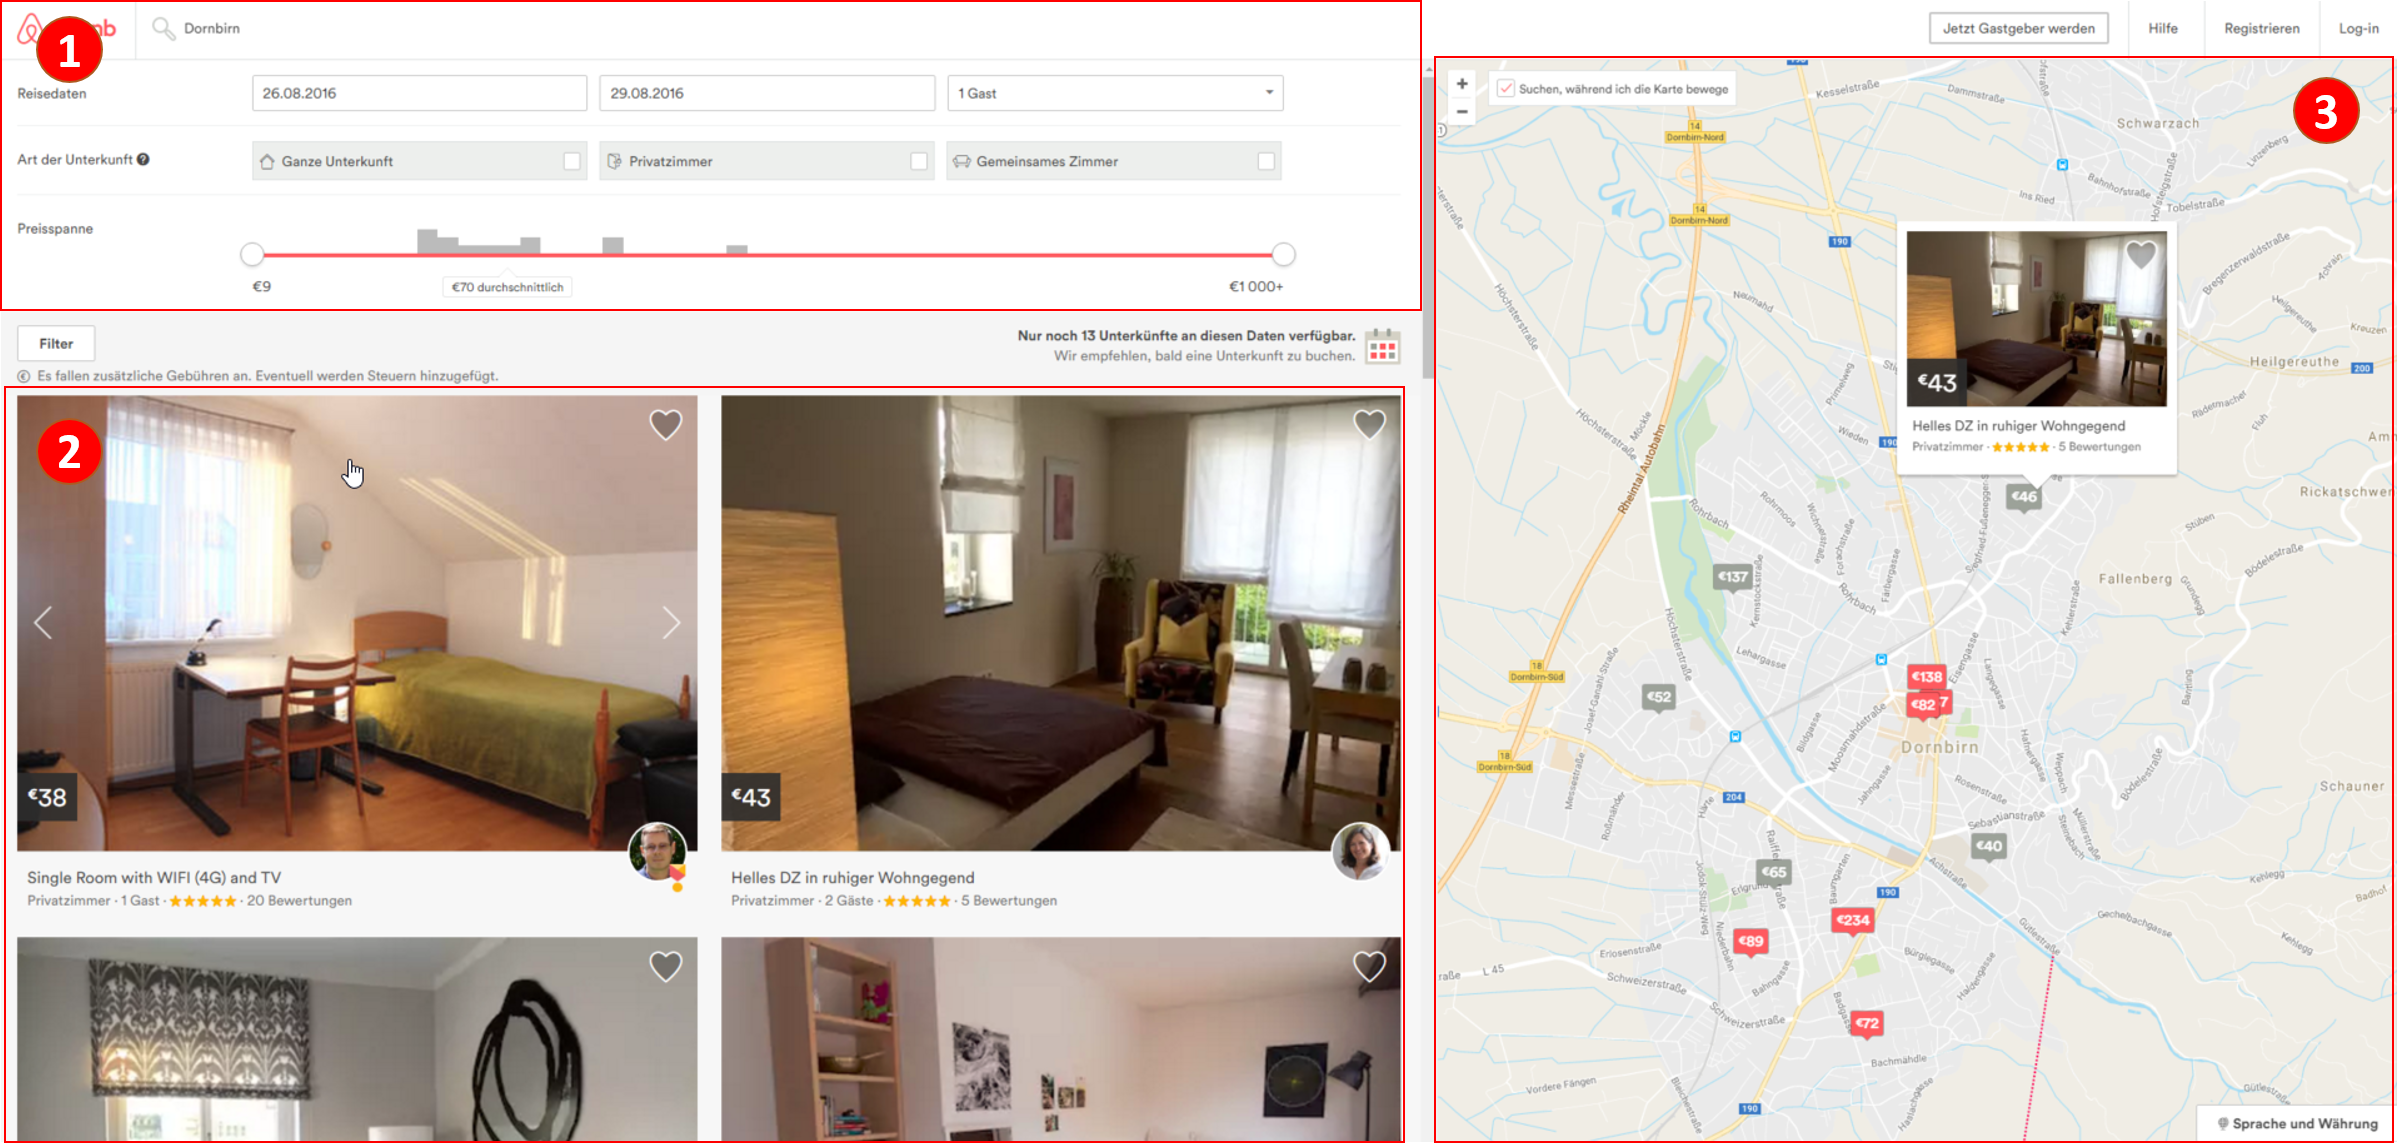
\includegraphics[width=1\linewidth]{img/StandDerTechnik/airbnbOverview}
\caption[kurz]{lang}
\label{fig:airbnbOverview}
\end{figure}

\begin{figure}[h]
\centering
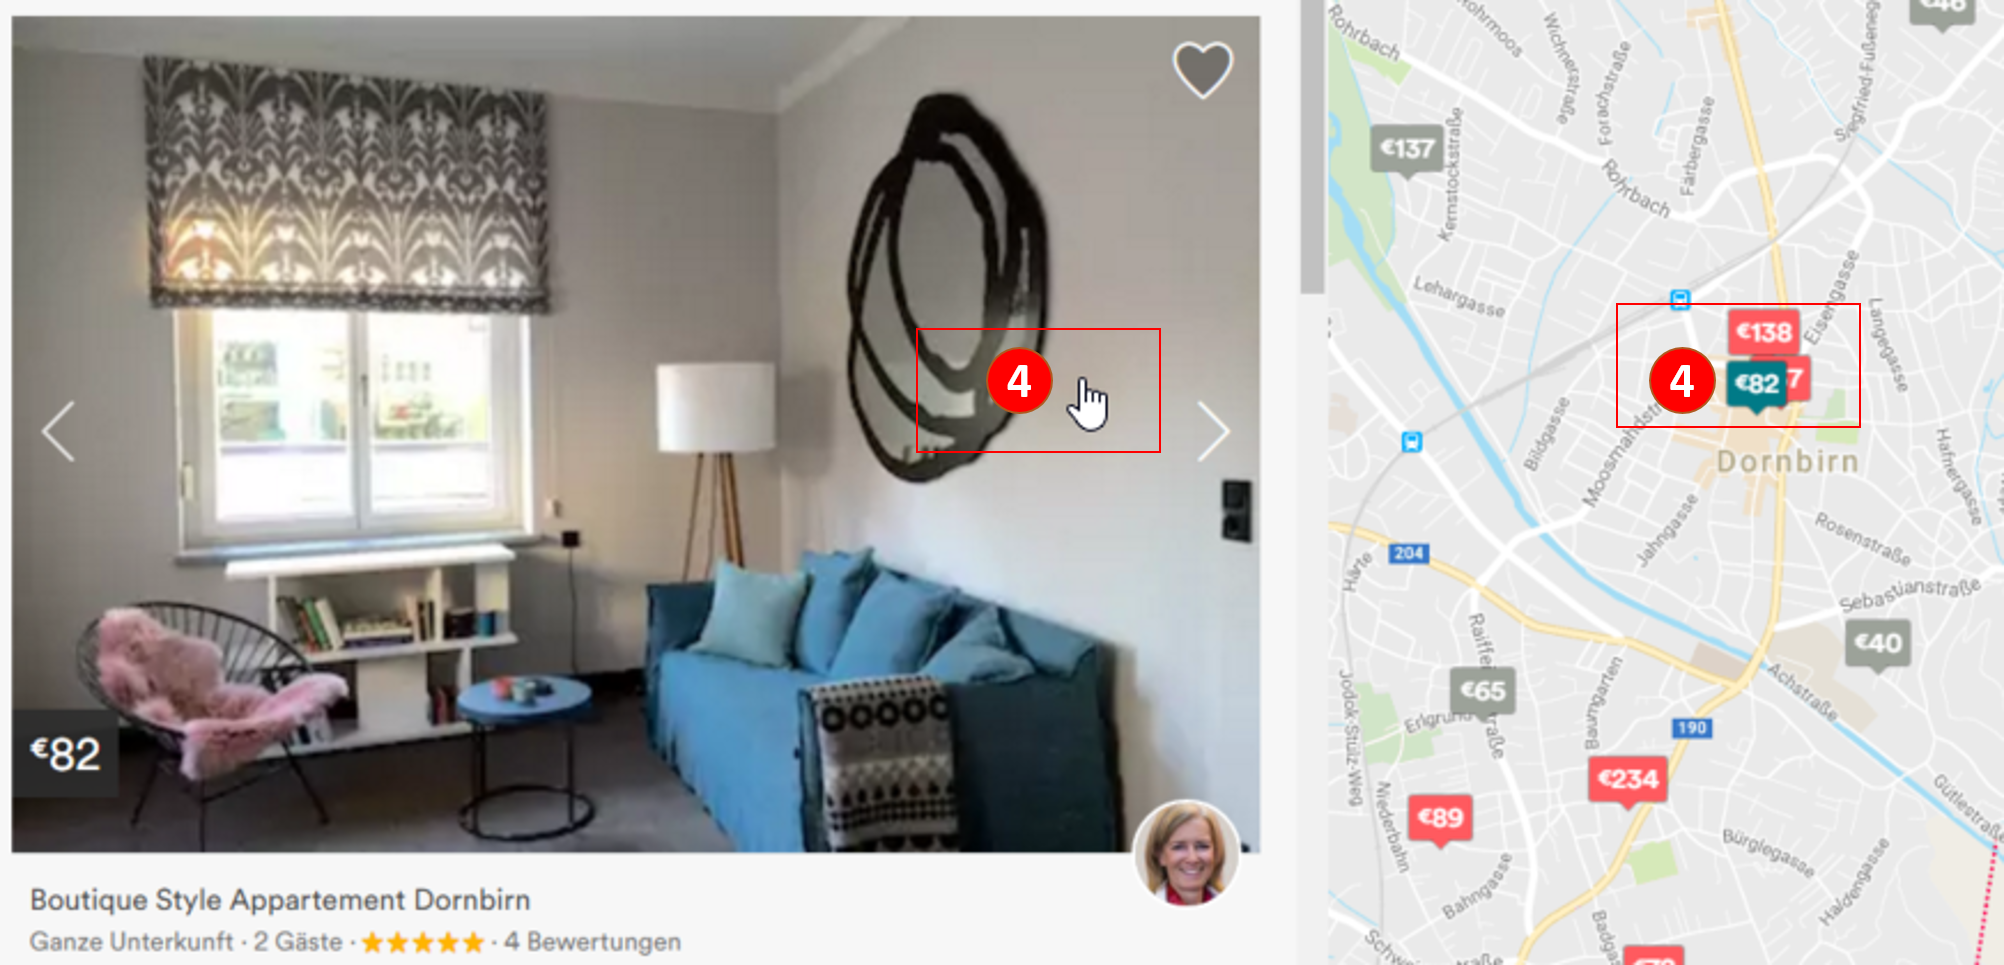
\includegraphics[width=1\linewidth]{img/StandDerTechnik/airbnbDetail}
\caption[kurz]{lang}
\label{fig:airbnbDetail}
\end{figure}


\subsection{Flightradar24}

\end{document}